\documentclass[10pt,a4paper]{article}
\usepackage[margin=2.2cm]{geometry}
\usepackage{fontspec}
\usepackage{kotex}
\setmainfont{Apple SD Gothic Neo}
\setsansfont{Apple SD Gothic Neo}
\usepackage{amsmath,amssymb}
\usepackage{graphicx}
\usepackage{booktabs}
\usepackage{caption}
\usepackage[dvipsnames]{xcolor}
\usepackage[colorlinks=true,linkcolor=MidnightBlue,citecolor=MidnightBlue,
            urlcolor=MidnightBlue]{hyperref}
\usepackage{titlesec}
\titleformat{\section}{\large\bfseries}{\thesection}{0.6em}{}
\titleformat{\subsection}{\normalsize\bfseries}{\thesubsection}{0.5em}{}
\captionsetup{font=small,labelfont=bf}
\setlength{\parskip}{0.35em}
\setlength{\parindent}{0pt}

\usepackage{mdframed}
\newmdenv[linewidth=0.4pt,linecolor=gray!60,backgroundcolor=gray!5,
          innertopmargin=6pt,innerbottommargin=6pt,skipabove=8pt,skipbelow=8pt]{claimbox}
\newcommand{\claim}[2]{\begin{claimbox}\textbf{주장.} #1\par\smallskip
  \textcolor{gray!70}{\textbf{반증 조건.} #2}\end{claimbox}}

\title{\bfseries 시간의 세금\\[2pt]
\large 같은 곡선, 반토막 난 세계 --- $n^{*}$ 는 남고 수준이 무너진다}
\author{월드모델 실험실 · 노트 $816$}
\date{2026-08-07}
\begin{document}\maketitle

\section{한 줄}

논문 $177$ 의 정직 조항을 이행했다 --- 같은 적응 곡선을 \textbf{시간
갈림}(평가 $=$ KR $2025{\sim}26$ 시작 $322$행 · 풀 $=$ 과거 $1{,}394$행)으로.

\begin{center}
\begin{tabular}{lrrr}
\toprule
& 무작위(논문 $177$) & \textbf{시간(이번)} & \\
\midrule
전이 기준선 & $0.6877$ & $\mathbf{0.2958}$ & $-57\%$ \\
단독 고원($n{=}800$) & $0.7507$ & $\mathbf{0.3383}$ & $-55\%$ \\
$n^{*}$ & $50$ & $\mathbf{50}$ & \textbf{불변} \\
\bottomrule
\end{tabular}
\end{center}

판정은 같다(3.교차 · $n^{*}{=}50$ · 두 번째 이행도 충돌 없음). \textbf{그러나
진짜 발견은 붕괴다} --- 시간 이동이 전이도 단독도 반토막 낸다.

\begin{figure}[t]\centering
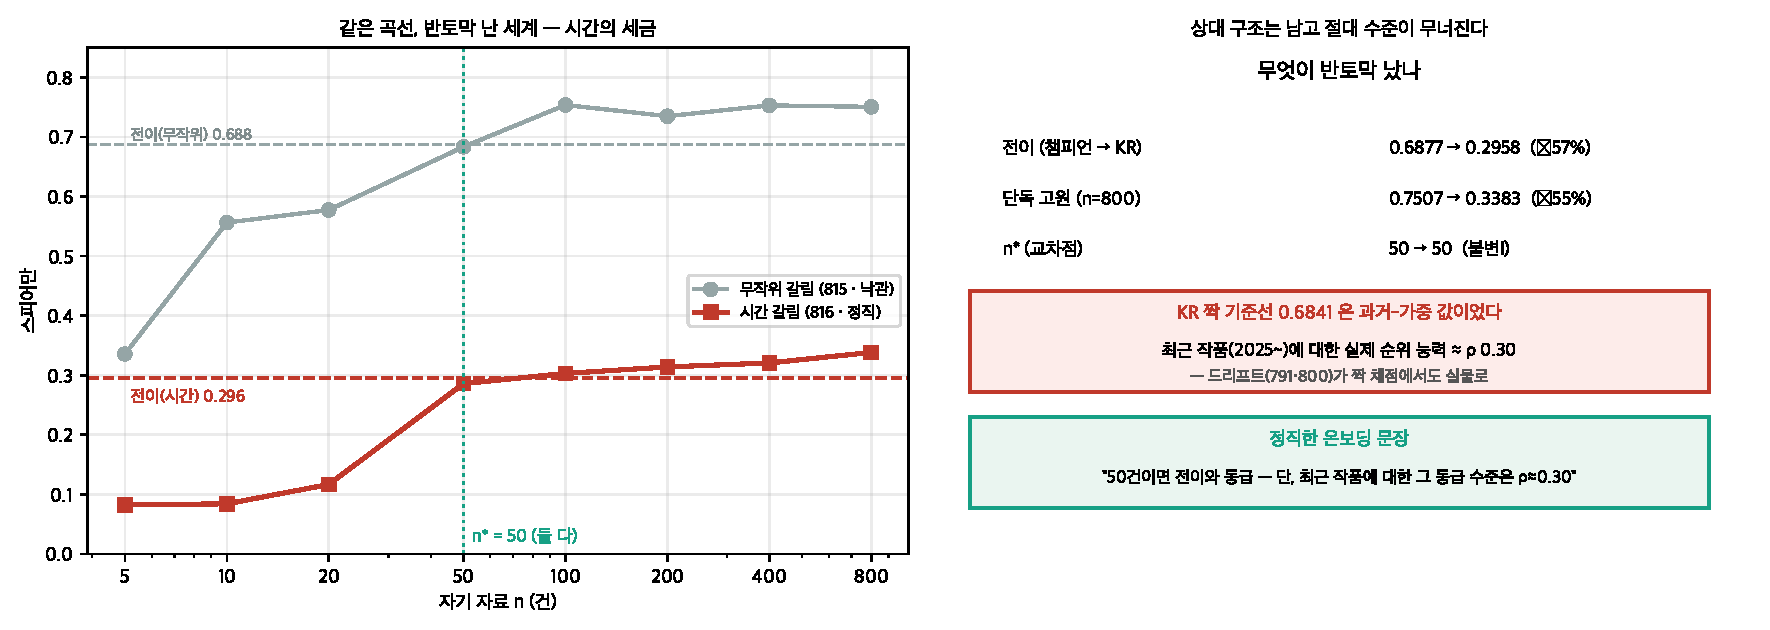
\includegraphics[width=0.97\textwidth]{figs/tax.pdf}
\caption{왼쪽: 두 세계의 같은 곡선. 오른쪽: 반토막 표와 정직한 문장.}
\end{figure}

\section{KR 짝 기준선은 과거-가중 값이었다}

\claim{\textbf{$0.6841$(짝 자 · 규약 $12$ 의 그 숫자)은 과거 행이 끌던 값이다.}
최근 작품($2025{\sim}$)만 채점하면 챔피언 전이가 $\mathbf{0.2958}$ 이다 ---
노트 $791 \cdot 800$ 의 드리프트(\emph{예보는 새 행에서 눌린다})가 짝 채점에서도
실물로 섰다. \textbf{함의 둘}: ① 온보딩 문장에는 \emph{절대 수준 병기가
의무}다 --- ``$50$건이면 전이와 동급''은 참이지만 \emph{그 동급이 최근 작품에서
$\rho \approx 0.30$} 이라는 것을 같이 말해야 한다(자릿수·구간 능력과 같은 정직
방식). ② 논문 $157$ 의 $0.0002$ 미달 서사가 새 조명을 받는다 --- 그 문턱
싸움 전체가 \emph{과거-가중 자} 위에서 벌어졌다.}
{$n^{*}{=}50$ 이 두 갈림에서 같다는 것은 \textbf{상대 구조(교차점)는 시간에
강건}하다는 뜻이다 --- 무너진 것은 절대 수준이지 곡선의 모양이 아니다. 그리고
단독이 $n{=}800$ 에서 전이를 $+0.042$(뽑기 SD 의 약 $2$배) 넘는 방향도
유지된다 --- 크기만 $+0.065 \to +0.042$ 로 줄었다.}

\section{예측 채점}

주 갈래(교차) 적중 · $n^{*}$ 는 두 번 연속 내 구간 밖($50$) · \textbf{전이
기준선 붕괴는 예측했으나 크기에 놀랐다}($0.68$ 아래로 --- 실제 $-0.39$).
\emph{적었던 것보다 세상이 더 그랬다.} T$1$ 의 측정 갈래가 이것으로 소진됐다 ---
적응 곡선 완결($815 \cdot 816$) · 남은 문은 수집. 판 $\rho$ $0.4689$ 그대로.

\end{document}
